\section{Theorie}
\label{sec:Theorie}
Mikrowellen sind elektromagnetische Wellen in einem Frequenzbereich von $300$ MHz bis 300 GHz. Durch
Hohlleiter lassen sich Mikrowellen verlustarmer übertragen als bei anderen Leitern, da
sie im Inneren Luft als Medium besitzen. Hohlleiter können verschieden Formen haben,
jedoch wird in diesem Versuch lediglich ein rechteckförmiger verwendet. Der Hohlleiter
kann die verschiedene Wellentypen, welche Moden genannt werden, leiten. Jeder Modus hat
eine bestimmte elektrische- und magnetische Feldverteilung. Bei einem TE-Modus ist das elektrische
Feld senkrecht zur Hohlleiterachse ausgerichtet und bei einem TM-Modus das magnetische Feld.
Die Moden haben eine Grenzfrequenz $f_c$, sodass
bei kleineren Frequenzen keine Energie mehr transportiert werden kann.

\subsection{Erzeugung von Mikrowellen}
Die Mikrowellen werden durch ein Reflexklystron erzeugt. In diesem treten Elektronen
aus einer Kathode aus und werden auf einen Hohlraumresonator beschleunigt. An diesem
wird eine Spannung angelegt, sodass ein LC-Schwingkreis ein Hochfrequenzfeld erzeugt.
Durch dieses Feld werden die Elektronen  bei dem Durchlaufen des Resonators teilweise beschleunigt und abgebremst.
Hinter dem Resonator treffen die Elektronen auf einen Reflektor, wodurch deren
Bewegungsrichtung umgekehrt wird und diese erneut den Hohlraumresonator durchlaufen.
Durch das Umkehren der unterschiedlich schnellen Elektronen, dem Anlegen von verschiedenen Reflektorspannungen und dem Ändern
des Resonatorvolumens , formen sich die Elektronen zu Bündeln und
geben beim Abbremsen in dem Resonator Energie an den Schwingkreis ab, wodurch dieser
aufrechterhalten wird. Dadurch kann die Frequenz der Mikrowellen moduliert werden. Die Energie des Schwingkreises wird induktiv ausgekoppelt und
durch einen Hohlleiter transportiert. In Abbildung (1) ist der Aufbau
eines Reflexklystrons dargestellt.

\begin{figure}[H]
  \centering
  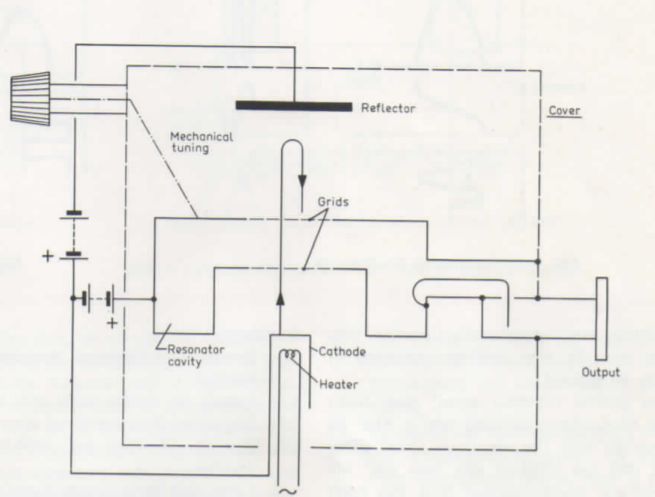
\includegraphics[height=6cm]{klystron.PNG}
  \caption{Aufbau eines Reflexklystron \cite{sample1}}
  \label{fig:Lock}
\end{figure}

\subsection{Frequenz, Wellenlänge und Dämpfung in einem Hohlleiter}
Für die Wellenlängen im freien Raum $\lambda_0$ und in einem Hohlleiter $\lambda_g$ gilt:

\begin{align}
  \lambda_0 &= \frac{c}{f} \\
  \lambda_g &= \frac{\lambda_0}{\sqrt{1- \left( \frac{\lambda_0}{\lambda_c} \right)^2}}
\end{align}

Hierbei ist $\lambda_c$ die Grenzwellenlänge, $c$ die Lichtgeschwindigkeit und $f$
die Frequenz der Welle. Für den TE-oder TM-Modus gilt für die
Grenzwellenlänge:

\begin{align}
  \lambda_c = \frac{2}{\sqrt{\left(\frac{m}{a} \right)^2 - \left(\frac{n}{b} \right)^2}}
\end{align}

mit den Moden $m$ und $n$, sowie den Maßen des rechteckigen Hohlleiters $a$ und $b$.
Mit diesen Gleichungen folgt, unter der Bedingung $\lambda_c=2a$, für die Frequenz:
\begin{align}
  f = \frac{c}{\lambda_0} = c \cdot \sqrt{\left(\frac{1}{\lambda_g}\right)^2 - \left(\frac{1}{2a}\right)^2}
\end{align}


%Die Dämpfung $D$ kann sowohl aus einem Leistungsverhältnis als auch einem Spannungsverhältnis berechnet werden:
%\begin{align}
%  D = 10  \ln{\frac{P_1}{P_2}} = 20 \ln{\frac{U_1}{U_2}}
%\end{align}
%\cite{sample}


\subsection{Bestimmung des Stehwellenverhältnisses}
Die durch den Hohlleiter laufenden Mikrowellen können an Fehlstellen teilweise reflektiert
werden, wodurch sie mit sich selbst überlagern und eine stehende Welle ausbilden können.
Für eine maximale stehende Welle müssen Phasen und Amplituden der überlagernden Wellen
gleich sein. Das Stehwellenverhältnis (SWR) ist dann als Verhältnis zwischen maximaler
und minimaler Feldstärke auf der Leitung definiert. Für das Bestimmen des Stehwellenverhältnisses
sind drei unterschiedliche Methoden möglich.

\textbf{1.} Das SWR kann direkt durch eine Sonde gemessen werden, wobei nur kleine SWR
damit genau gemessen werden können, da die Sonde das elektrische Feld sonst stärker
stört.

\textbf{2.} Es werden die beiden Ausgangsspannungen gemessen, welche den doppelten Wert
des Minimums haben. Für das SWR gilt dann:

\begin{align}
  &S = \sqrt{1+  \left(\frac{1}{\sin^2{ \frac{\pi(d_1 - d_2)}{\lambda_g} }} \right) } \\
  &S = \frac{\lambda_g}{\pi(d_1-d_2)} \: \:\:\: \text{für} \:S > 10
\end{align}

\textbf{3.} Wird mit einem Dämpfer das Maximum des Ausgangssignals dem Minimum gleichgemacht, gilt:
\begin{align}
  A_2 - A_1 = 20 \log_{10}(S)
\end{align}
Wobei $A_2 - A_1$ die Differenz der Einstellungen des Abschwächers ist.
